\documentclass[12pt]{article}
\usepackage{pdfpages}
\parindent=0pt
\parskip=\bigskipamount
\begin{document}
\begin{center} Math 2710: Transition to Advanced Math \\
Jeremy Teitelbaum \\ Fall Semester, 2019
\end{center}

{\bf Instructor}\\
Jeremy Teitelbaum \\
{\tt jeremy.teitelbaum@uconn.edu} \\
{\tt http://teitelbaum.math.uconn.edu} \\
Office: Monteith 231 \\
Office hours: 9:00 - 10:00 Mondays, 12:15-13:00 Wednesdays (or by appointment) \\


{\bf Course Description.} This course is an introduction to mathematical proof, taught through examples mainly from
algebra and number theory.  

{\bf Textbook:} An Introduction to Mathematical Thinking: Algebra \& Number Systems, by Gilbert and Vanstone. Pearson, New Jersey.
ISBN 0-13-184868-2.

{\bf Prerequisites.} MATH 1132 or 1152. Cannot be taken for credit after passing MATH 2143, 3150, 3210, 3230, 3240, 3260, 3270, 3330, 3370 or 224. 

{\bf Piazza.}  We will be using the piazza Q\&A site for intra-class consultation.  Questions about the course should be directed to the piazza site. Course resources are also available through piazza.  You can access piazza through the Husky CT course for the class, but you should have received an email enrolling you in the class and providing a direct link.

\vfill\eject

{\bf Assessment.}  Grades in this course will be based on the
following:
\begin{itemize}
\item $2$ midterm exams, each worth $25\%$ of the total grade.
Tentatively scheduled for September 30 and November 5. Note: September
30 is Rosh Hashanah.  If you are celebrating the holiday, \textit{see
me by September 20} to sign up for an alternate exam date, probably
October 3.
\item Final Exam worth $40\%$ of the final grade.
\item Homework and Participation (10\%).  I will assign a number of
homework problems for discussion in each class, and you should do
these homework problems before class and come prepared to discuss
them.  Periodically, I will select a subset of the assigned problems
to be handed in.  I will provide relatively little lead time for these
assignments so it is in your interest to stay current. You may
collaborate or use piazza when completing this work, but the final
write-up must be your own work.  In addition, I may from time to time
make and grade other assignments including short in-class or online
quizzes, and I will explain the rules for collaboration on those
problems when they happen.
\item Piazza.  Part of your homework and participation grade depends
on your use of piazza.  Prior to (most) classes, I will post a
question or discussion topic to piazza pertaining to the next class.
You should take the time to respond to these posts; each such question
will count roughly the same as a typical homework problem or in-class
quiz question.
\end{itemize}

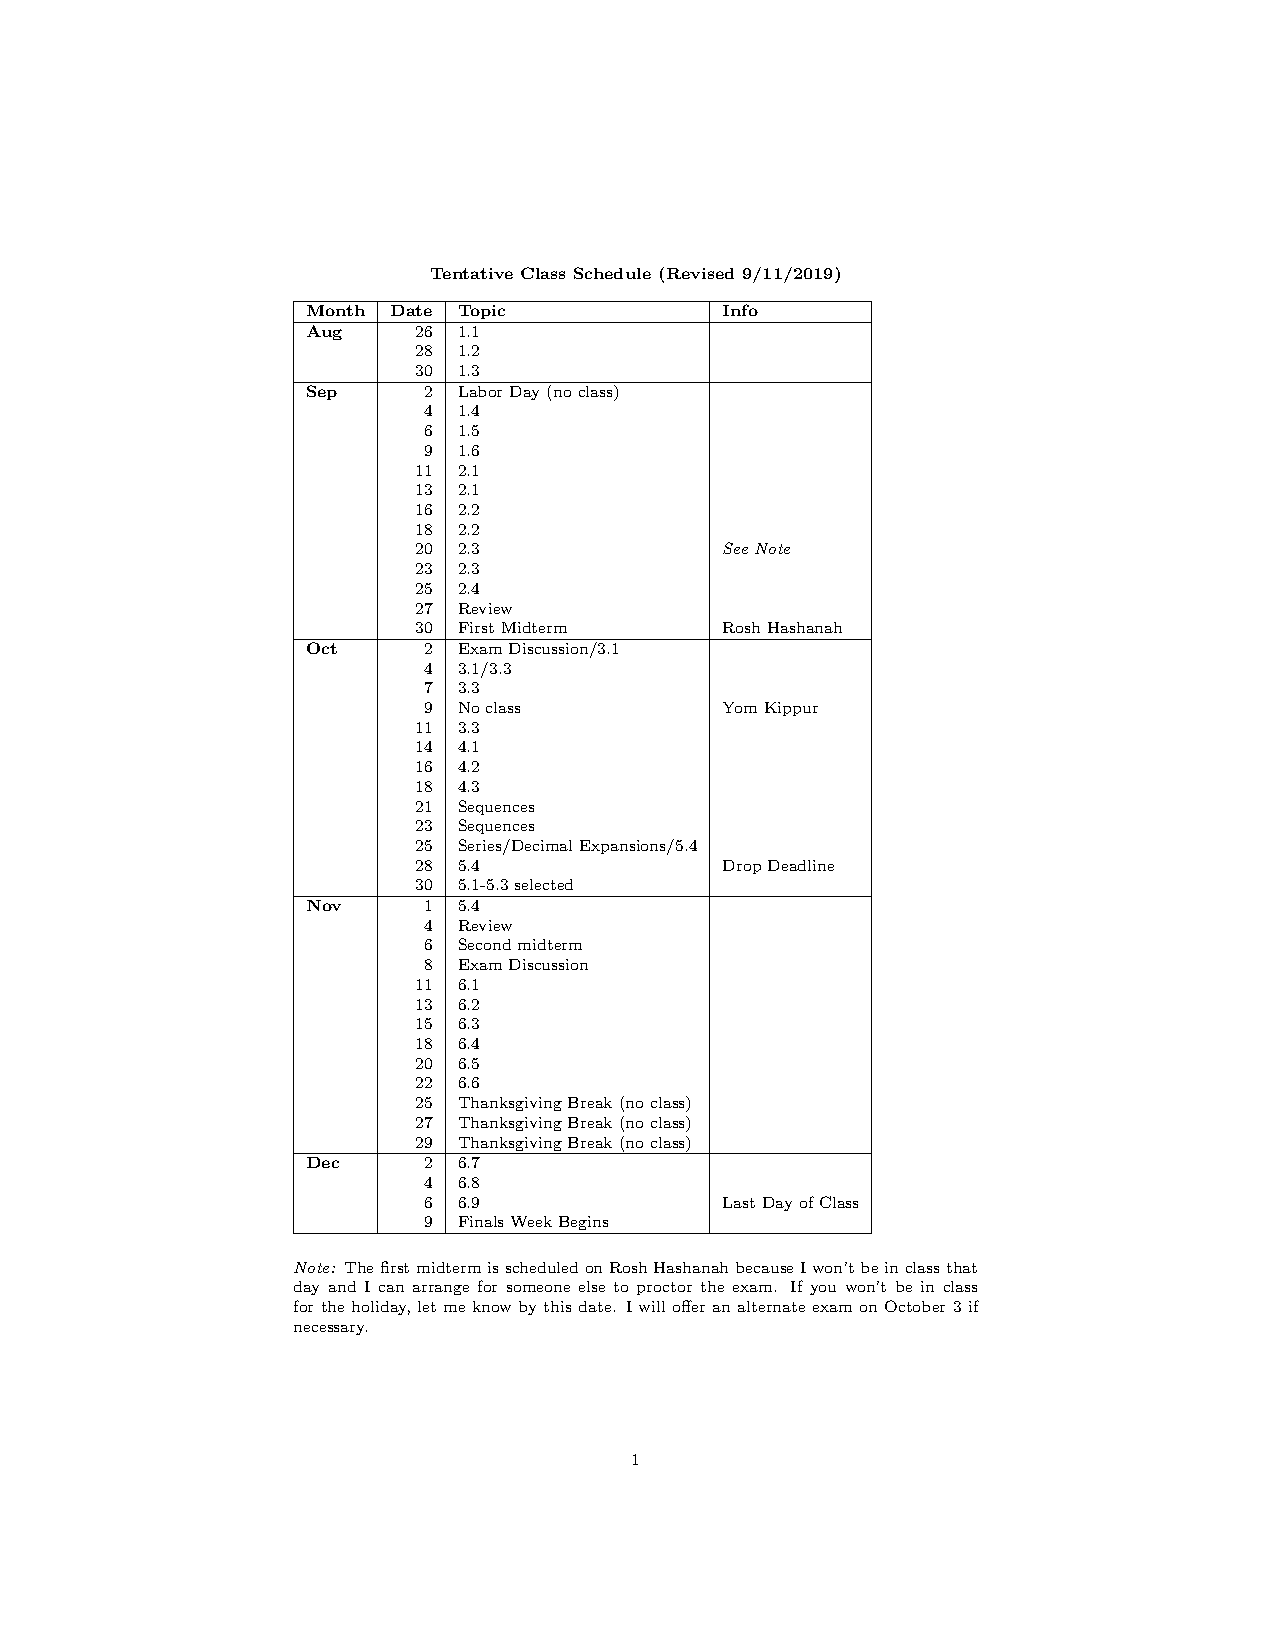
\includepdf{schedule.pdf} 

\begin{center}

{\Large Policy Statements}

\end{center}

{\bf Academic Integrity} 

Students are bound by the university's policies on academic integrity.

{\bf Students with Disabilities}

{\it Students with disabilities} should contact Teitelbaum as soon as
possible to discuss any accommodations needed during the semester due
to a documented disabilities.  If you have a documented disability for
which you wish to request academic accommodations and have not
contacted the Center for Students with Disabilities, please do so as
soon as possible.  The CSD is located in Wilbur Cross, Room 204 and
can be reached at (860) 486-2020 or at csd@uconn.edu.  Detailed
information regarding the process to request accommodations is
available on the CSD website at www.csd.uconn.edu.

{\bf Policy Against Discrimination, Harassment and Inappropriate
Romantic Relationships}

The University is committed to maintaining an environment free of
discrimination or discriminatory harassment directed toward any person
or group within its community – students, employees, or visitors.
Academic and professional excellence can flourish only when each
member of our community is assured an atmosphere of mutual respect.
All members of the University community are responsible for the
maintenance of an academic and work environment in which people are
free to learn and work without fear of discrimination or
discriminatory harassment.  In addition, inappropriate Romantic
relationships can undermine the University’s mission when those in
positions of authority abuse or appear to abuse their authority.  To
that end, and in accordance with federal and state law, the University
prohibits discrimination and discriminatory harassment, as well as
inappropriate Romantic relationships, and such behavior will be met
with appropriate disciplinary action, up to and including dismissal
from the University.  More information is available at
http://policy.uconn.edu/?p=2884.

{\bf Sexual Assault Reporting Policy}

To protect the campus community, all non-confidential University
employees (including faculty) are required to report assaults they
witness or are told about to the Office of Diversity \& Equity under
the Sexual Assault Response Policy.  The University takes all reports
with the utmost seriousness.  Please be aware that while the
information you provide will remain private, it will not be
confidential and will be shared with University officials who can
help.  More information is available at
http://sexualviolence.uconn.edu/.


\end{document}




%%% Local Variables:
%%% mode: latex
%%% TeX-master: t
%%% End:
